%%%%%%%%%%%%%%%%%%%%%%%%%%%%%%%%%%%%%%%%%
% Large Colored Title Article
% LaTeX Template
% Version 1.1 (25/11/12)
%
% This template has been downloaded from:
% http://www.LaTeXTemplates.com
%
% Original author:
% Frits Wenneker (http://www.howtotex.com)
%
% License:
% CC BY-NC-SA 3.0 (http://creativecommons.org/licenses/by-nc-sa/3.0/)
%
%%%%%%%%%%%%%%%%%%%%%%%%%%%%%%%%%%%%%%%%%

%----------------------------------------------------------------------------------------
%	PACKAGES AND OTHER DOCUMENT CONFIGURATIONS
%----------------------------------------------------------------------------------------

\documentclass[DIV=calc, paper=letter, fontsize=10pt, twocolumn]{scrartcl}	 % A4 paper and 11pt font size

\usepackage{graphicx}
\usepackage{hyperref}
\usepackage{lipsum} % Used for inserting dummy 'Lorem ipsum' text into the template
\usepackage[english]{babel} % English language/hyphenation
\usepackage[protrusion=true,expansion=true]{microtype} % Better typography
\usepackage{amsmath,amsfonts,amsthm} % Math packages
\usepackage[svgnames]{xcolor} % Enabling colors by their 'svgnames'
\usepackage[hang, small,labelfont=bf,up,textfont=it,up]{caption} % Custom captions under/above floats in tables or figures
\usepackage{booktabs} % Horizontal rules in tables
\usepackage{fix-cm}	 % Custom font sizes - used for the initial letter in the document
\usepackage{booktabs}
\usepackage{paralist}

\usepackage{sectsty} % Enables custom section titles
\allsectionsfont{\usefont{OT1}{phv}{b}{n}} % Change the font of all section commands

\usepackage{fancyhdr} % Needed to define custom headers/footers
\pagestyle{fancy} % Enables the custom headers/footers
\usepackage{lastpage} % Used to determine the number of pages in the document (for "Page X of Total")

% Headers - all currently empty
\lhead{}
\chead{}
\rhead{}

% Footers
\lfoot{}
\cfoot{}
\rfoot{\footnotesize Page \thepage\ of \pageref{LastPage}} % "Page 1 of 2"

\renewcommand{\headrulewidth}{0.0pt} % No header rule
\renewcommand{\footrulewidth}{0.4pt} % Thin footer rule

\usepackage{lettrine} % Package to accentuate the first letter of the text
\newcommand{\initial}[1]{ % Defines the command and style for the first letter
\lettrine[lines=3,lhang=0.3,nindent=0em]{
\color{DarkGoldenrod}
{\textsf{#1}}}{}}

%----------------------------------------------------------------------------------------
%	TITLE SECTION
%----------------------------------------------------------------------------------------

\usepackage{titling} % Allows custom title configuration

\newcommand{\HorRule}{\color{DarkGoldenrod} \rule{\linewidth}{1pt}} % Defines the gold horizontal rule around the title

\pretitle{\vspace{-30pt} \begin{flushleft} \HorRule \fontsize{50}{50} \usefont{OT1}{phv}{b}{n} \color{DarkRed} \selectfont} % Horizontal rule before the title

\title{\Huge Literature Search Made Easy} % Your article title

\posttitle{\par\end{flushleft}\vskip 0.5em} % Whitespace under the title

\preauthor{\begin{flushleft}\large \lineskip 0.5em \usefont{OT1}{phv}{b}{sl} \color{DarkRed}} % Author font configuration

\author{Bo Wang, Min Liu } % Your name

\postauthor{\footnotesize \usefont{OT1}{phv}{m}{sl} \color{Black} % Configuration for the institution name
\{bowang, liumin\}@stanford.edu % Your institution

\par\end{flushleft}\HorRule} % Horizontal rule after the title

\date{} % Add a date here if you would like one to appear underneath the title block

%----------------------------------------------------------------------------------------

\begin{document}

\maketitle % Print the title

\thispagestyle{fancy} % Enabling the custom headers/footers for the first page 

%----------------------------------------------------------------------------------------
%	ABSTRACT
%----------------------------------------------------------------------------------------

% The first character should be within \initial{}
\initial{M}\textbf{any of us have been faced with this situation: we found a certain field of research intriguing, went to an online archive to search for related papers, and the results were just less than satisfactory: they are too unstructured to obtain a big picture, such as how this field evolves over time, what sub-fields it is composed of. Instead of relying on human instinct for such insights, our project provides an alternative: using machine learning algorithms to peruse thru online archives, generate the information of interest, and present them in a human friendly way. In this project, we used hierarchical latent Dirichlet allocation (hLDA) to find the topics and their hierarchy and dynamic topic model (DTM) to find the time evolution of topics. In addition to using these two models, we also made an important extension to them, i.e. constructing the corpus with "key phrases" instead of "keywords" . Furthermore, we devised an algorithm to remove the duplication in word and phrase count, which enabled us to generate a corpus composed of both keywords and "key phrases". This approach allowed us to greatly improve the interpretability of the result since a large number of concepts in science and technology are formulated as phrases.\\
In our experiments with 14185 condensed matter physics papers from arXiv, the above methods effectively found the trend and hierarchy of research topics and revealed some very interesting insights. In our report, the "Trends in Research Topics" section demonstrates the analysis of topic trends, advantage of using "key phrases" versus keywords and a caveat in word and phrase count when constructing the corpus. The "Topic Hierarchy" section presents the generation of a hierarchy of topics and the solution to the caveat aforementioned.}
%----------------------------------------------------------------------------------------
%	ARTICLE CONTENTS
%----------------------------------------------------------------------------------------


\section*{Background}

\subsection*{Latent Dirichlet Allocation (LDA)}
Latent Dirichlet Allocation (LDA) \cite{1} is a Bayesian generative probabilistic model of a corpus. It assumes that documents are random mixtures of latent topics, where each topic is characterized by a distribution over words. Here we describe the smoothed LDA since this is the version of LDA that serves as the basis of the other models used in this paper.
Smoothed LDA assumes the following generative process (Figure ~\ref{fig: LDA}) for a document in a corpus D:
\begin{enumerate}
  \item Choose $N \sim Poisson(\xi)$.
  \item Choose $\theta \sim Dir(\alpha)$.
  \item Choose $\beta \sim Dir(\eta)$.
  \item For each of the N words $w_n$:
  	\begin{enumerate}
  	  	\item Choose a topic $z_n \sim  Multinomial(\theta)$
    		\item Choose a word $w_n$ from $p(w_n|z_n, \beta)$, a multinomial probability conditioned on the topic $z_n$.
  	\end{enumerate}
\end{enumerate}
The key computational problem of LDA is to infer the hidden variables, i.e. finding what hidden topic structure is most likely to generate the observed corpus with the above generative process. Once the posterior of the hidden variables are computed, it can be used to output topics words that appear most often in each topic. Details of the algorithm can be found in \cite{1}.
			\begin{figure}[!ht]
				\centerline{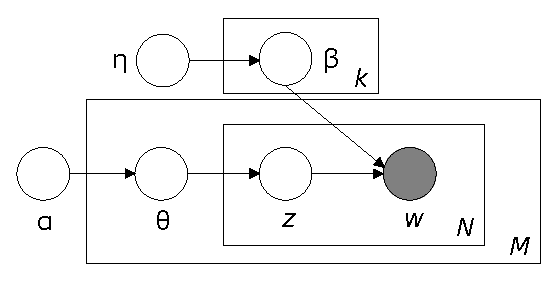
\includegraphics[scale = 0.8]{BleiNgJordan2003.eps}}
				\caption{Illustration of generative process of LDA \cite{1}}
				\label{fig: LDA}
			\end{figure}

\subsection*{Hierarchical Latent Dirichlet Allocation (hLDA)}
Hierarchical Latent Dirichlet Allocation (hLDA) \cite{2} is an extension of LDA which analyzes hierarchies of topics in a corpus. Instead of constraining each document to have a fixed finite number of k topics as LDA does, it allows an infinite number of topics, which are organized in a hierarchy, with the most abstract topics near the root of the hierarchy and more concrete topics near the leaves. In hLDA, a word is generated not based on the topic but a path of topics (from the root topic to the leaf topic) it belongs to.\newline
The generative process (Figure ~\ref{fig: hLDA})can be illustrated as:
\begin{enumerate}
  \item Let $c_1$ be the root topic.
  \item For each level $l \in 2,\ldots, L$ :
  	\begin{enumerate}
		\item Draw a sub-topic from topic $c_{l - 1}$.
		\item Set $c_l$ to be that sub-topic.
	\end{enumerate}

  \item Draw an L dimensional topic proportion vector $\theta$ from $Dir(\alpha)$.
  \item For each word $n \in \{ 1, \ldots, N \}$:
  	\begin{enumerate}
  	  	\item Draw $z \in \{ 1, \ldots, L \}$ from {\it Multinomial($\theta$)}.
    		\item Draw $w_n$ from the topic associated with $c_z$.
  	\end{enumerate}
\end{enumerate}
where the root topic is the topic on level 1, its sub-topics are those on level 2, etc.
			\begin{figure}[!ht]
				\centerline{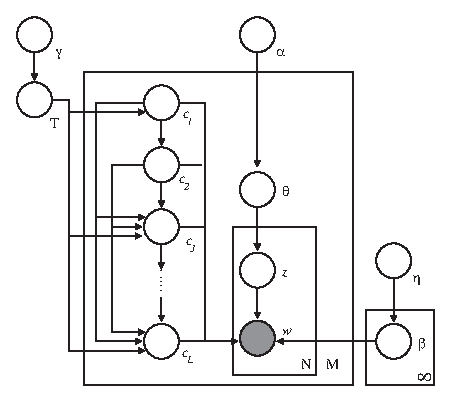
\includegraphics[scale = 0.8]{hLDA_paper.eps}}
				\caption{Illustration of generative process of hLDA \cite{2}}
				\label{fig: hLDA}
			\end{figure}

\subsection*{Dynamic Topic Model (DTM)}
Dynamic topic models (DTM) \cite{3} can be seen as a combination of LDA and time series. It is a generative model that analyzes the time evolution of topics of a collection of documents over time.\newline
The generative process of DTM (Figure~\ref{fig: DTM}) is as follows, where time t is discretized in to time slices:
\begin{enumerate}
  \item Draw topics $\beta_{t} |\beta_{t - 1} \sim N(\beta_{t-1}, \sigma^2I)$.
  \item Draw $\alpha_{t} |\alpha_{t - 1} \sim N(\alpha_{t-1}, \delta^2I)$.
  \item For each document:
  	\begin{enumerate}
  	  	\item Draw $\eta \sim N(\alpha_t, a^2I)$
    		\item For each word:
			\begin{enumerate}
  	  			\item Draw $Z \sim Multinomial(\pi(\theta))$.
    				\item Draw $W_{t,d,n} \sim Multinomial(\pi(\beta_{t,z})$, with $\pi(\beta_{k,t})_w = \frac{exp(\beta_{k,t,w})}{\sum_w exp(\beta_{k,t,w})}$
			\end{enumerate}
  	\end{enumerate}
\end{enumerate}
Here, $\beta$ and $\theta$ are not sampled from Dirichlet distributions as in smoothed LDA, instead, $\beta_{t,k}$ is a random walk with Gaussian steps, while $\theta$ is drawn from a logistic normal with mean $\alpha_t$, which undergoes similar dynamics as $\beta_{t,k}$. The choice of logistic normal is due to its amenability with time series modeling. \newline
DTM computes the posterior of hidden variables of all the time slices, which is used to output the evolution of topics and keywords.
\begin{figure}[!ht]
				\centerline{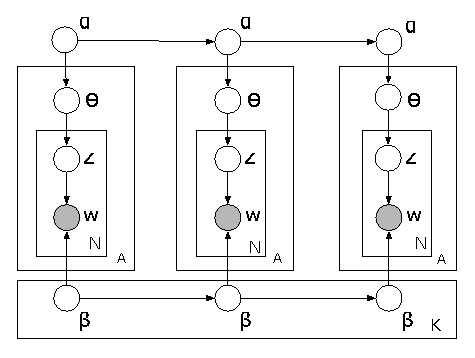
\includegraphics[scale = 0.8]{p113-blei.eps}}
				\caption{Illustration of generative process of DTM \cite{3}}
				\label{fig: DTM}
			\end{figure}

\section*{Feature Extraction}
\subsection*{Data Cleanse}
The collection of documents have to be converted to a term frequency matrix as required by all the topic models described above. Instead of generating a term matrix with raw data, we pre-process the data as follows to remove noise:
\begin{enumerate}
  \item Separate an abstract into sentences.
  \item For each sentence:
    	\begin{enumerate}
  	  	\item Remove stop words (e.g. 'the', 'and', 'of').
		\item Remove tokens containing no letters.
		\item Remove common verbs (e.g. 'get', 'take', 'think').
		\item Remove tokens shorter than minimum term length of 3 characters.
		\item Remove latex format tokens.
		\item Split hyphen connected words if both words are longer than the minimum term length.
		\item Convert nouns to sigular form and verbs to infinitive form.
		\item Stem tokens.
  	\end{enumerate}
\end{enumerate}
Then we generate a dictionary containing all terms that appeared in at least 5 documents and a term matrix whose ($i$, $j$)-th element n denotes that the $j$-th word in the dictionary occurred n times in the $i$-th document.
 
\subsection*{Phrase Generation}
While doing data pre-processing, we observed that new concepts in science and technology are usually expressed in the form of phrases, such as "computer science", "machine learning" and "topic modeling", which indicates a topic might be better characterized by its "key phrases" instead of keywords. Furthermore, phrases also offer better interpretability of results, e.g. a topic with keywords {"dimension", "principal", "analysis"} may greatly perplex us, while one with key phrases {"principal component analysis", "dimension reduction"} is quite informative.\newline
We generated phrases before the second step in the previous section by:
\begin{enumerate}
  \item Separate words into blocks by punctuation marks and stop words.
  \item Within each block, generate phrases made up of consecutive words while restricting the maximum length of phrases to 5 words since usually phrases longer than 5 words are represented by their acronyms.
\end{enumerate}
\subsection*{Duplicate Counts Removal}
Using the phrase generation method described above can lead to duplicate counts in the resulting corpus. For example, phrase "Stanford University" will generate "Stanford" once, "University" once and "Stanford University" once, while these two words should only be counted as a phrase once. To eliminate this inaccuracy, we implement a two-phase algorithm. The first phase is the same as the approach described above: extract words and enumerate phrases in each document, then filter the words and phrases whose occurrences are below the minimum threshold. In the second phase, documents are scanned through again. For each word in a document, we check whether it can be combined with its previous or next word to generate a phrase appearing in the filtered phrase dictionary. If not, this word is counted as one individual occurrence; otherwise it is skipped. This method basically recounts all terms and checks if their appearance contribute to the generation of a phrase. Only those terms not as part of a phrase is counted. By using this procedure, we were able to produce a corpus which nicely combines both phrases and words. 

\section*{Evaluation}

\subsection*{Experiment Setup}
Data is crawled from the online archive website arXiv. In fields like mathematics and physics, almost all scientific papers are self-archived on the arXiv. Despite not peer reviewed, arXiv has its submissions reviewed (or even recategorized if off-topic) by moderators that are experts in their fields of research. In addition, submission dates on arXiv more accurately reflect when the research project was completed and paper drafted, since usually papers are posted on arXiv months before they are finally published on a peer reviewed journal or conference. Based on these facts, we believe arXiv is a better collection of research works than any journal or conference alone.\newline
The titles, authors, abstracts and citation of papers are scraped from API of \url{http://export.arxiv.org/api/} using Python and stored in separate files according to the publish year. We used only papers in condensed matter physics since one of us is familiar to the field, the methods demonstrated in this report however can be applied to the analysis any field. The corpus contains 14185 abstracts from year 1992 to 2003 and 4645 unique words and 11255 unique phrases after our data processing procedure.


\subsection*{Results}
\subsubsection*{Trends in Research Topics}
In our DTM experiment, the number of topics is set to 10 a priori. Results are summarized in Figure ~\ref{fig: DTM_table_unweight} and Figure ~\ref{fig: PhaseTrans_wp}. In Figure ~\ref{fig: DTM_table_unweight} we demonstrate 5 out of the 10 topics for purpose of figure size control, the 3 tables respectively are topics and keywords generated from only words, words plus phrases and only phrases. In these tables, the topics are written in bold and keywords in regular font style. We see the in all cases, the DTM algorithm very nicely identifies major research topics. However, the classification with phrases only clearly gives much better interpretability. Note that the first two tables look quite similar, in fact, in the second table, even though the corpus contains both words and phrases, we can hardly see any phrases among the important keywords. This is quite intuitive since in the corpus, there are 486712 words, 4645 of them unique and 112448 phrases with 11250 of them unique. So on average, a word appears ~100 times in the corpus while a phrase appears only ~10 times, resulting in a term matrix dominated by words. This is what has motivated to remove the duplicated counts in words.
\begin{figure}[!ht]
  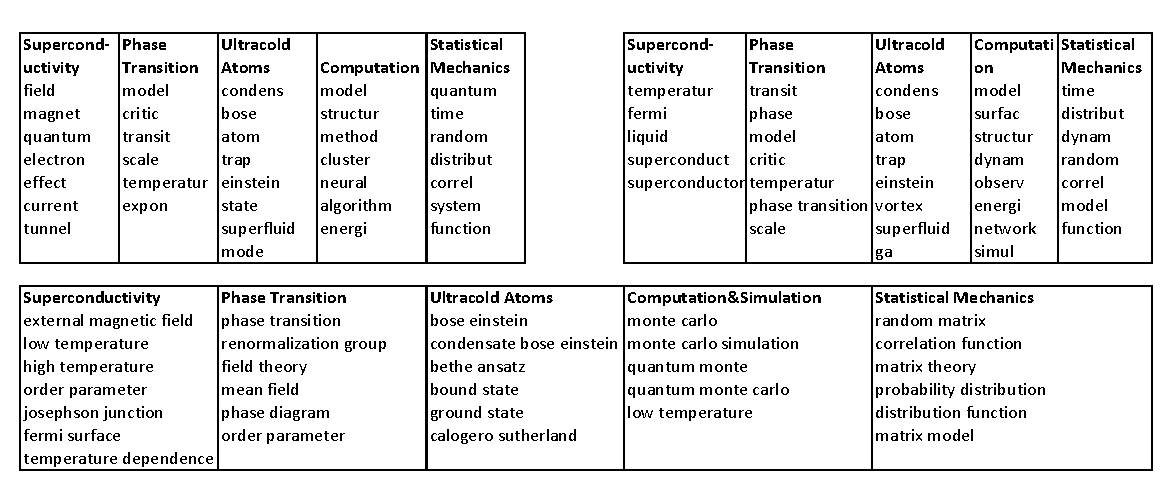
\includegraphics[scale = 0.45]{dtm10_unweight.eps}
  \caption{DTM Topics and Keywords. \rm{ Corpura corresponding to the 3 tables are respectively composed of a) words b) words plus phrases without removing duplicate counts c) phrases}}
  \label{fig: DTM_table_unweight}
\end{figure}
In Figure ~\ref{fig: PhaseTrans_wp}, we present the plot of one specific topic "phase transition", which is typical of all the plots.
\begin{figure}[!ht]
  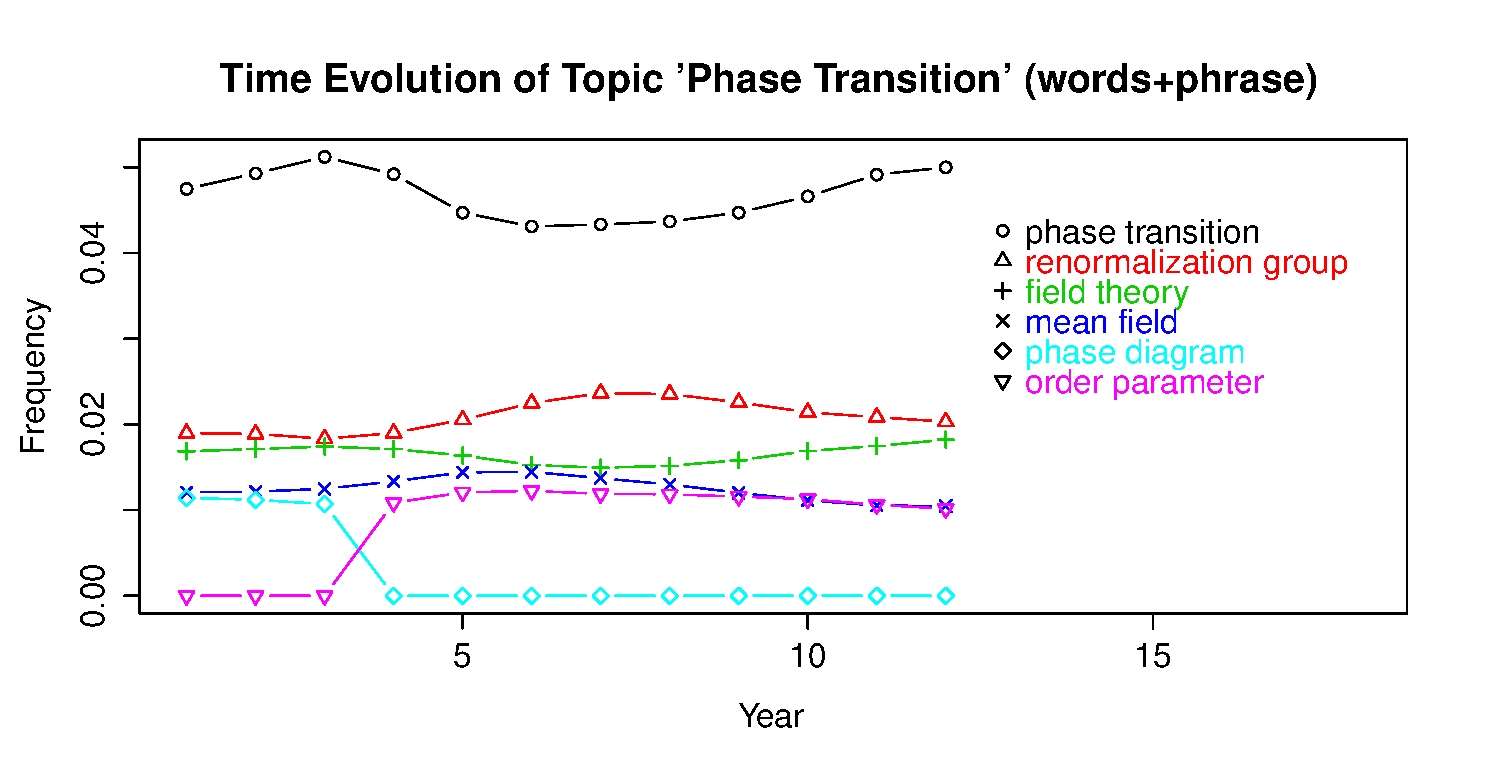
\includegraphics[scale = 0.365]{PhaseTrans(w_p).eps}
  \caption{Keywords Trend Plot of Topic "Phase Transition"}
  \label{fig: PhaseTrans_wp}
\end{figure}
From Figure ~\ref{fig: PhaseTrans_wp}, despite the frequencies of keywords do rise and fall, there is hardly any obvious "trend". This is not unexpected since it's natural that a paper on "phase transition" should always involve keywords such as "phase transition" and "phase diagram" regardless of when it is published.\newline
One very informative plot we can make is the evolution of topic popularity. In Figure ~\ref{fig: TopPop_p}, we show a plot of frequencies for 4 topics over time.
\begin{figure}[!ht]
  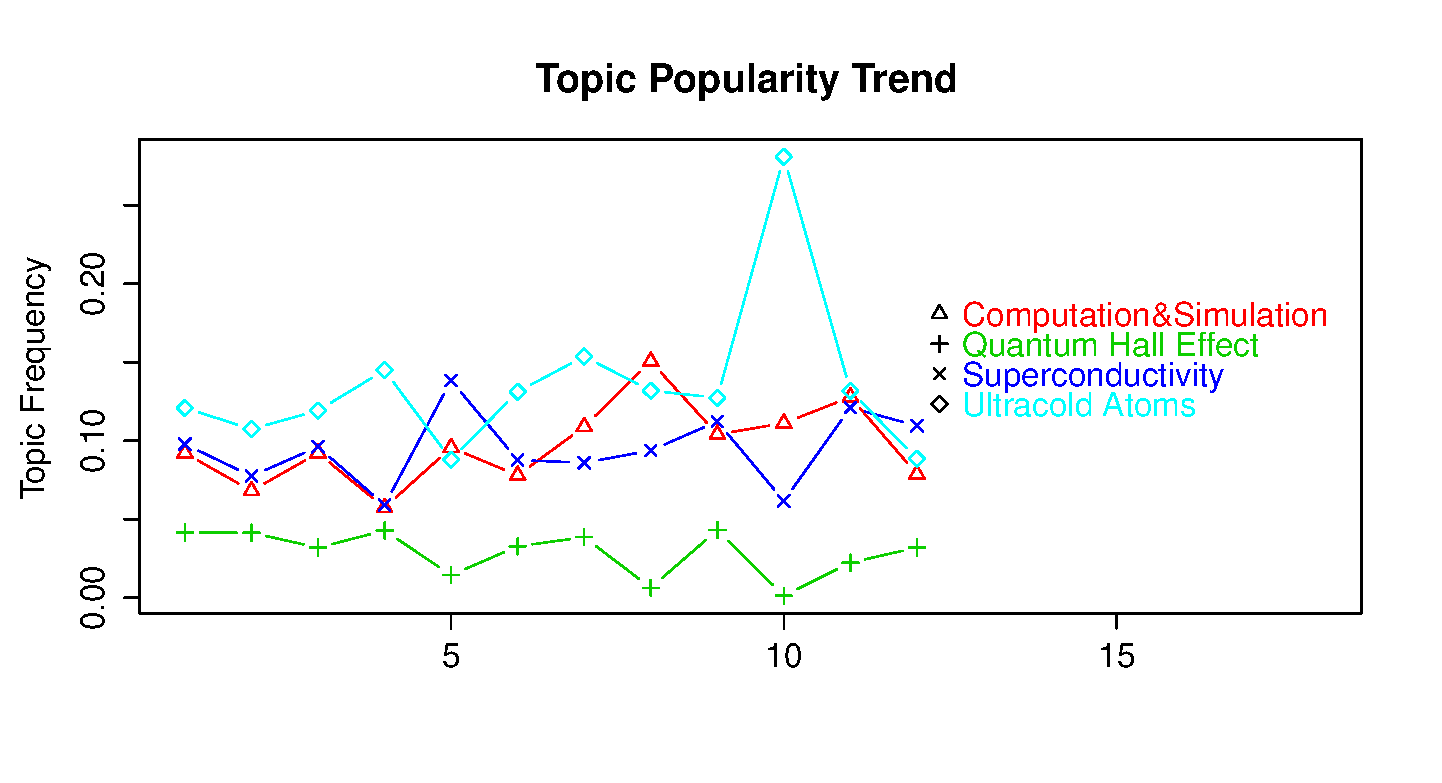
\includegraphics[scale = 0.365]{TopPop_p.eps}
  \caption{Plot of Frequencies of Different Topics over Time}
  \label{fig: TopPop_p}
\end{figure}
This plot has some really interesting implications: 
\begin{inparaenum}[\itshape a\upshape)]
\item "Superconductivity" and "Ultracold Atoms" are clearly negatively correlated, which indicates it is possible that for some reason (e.g. similarities in research techniques) research works in these two fields are almost done by the same group of researchers. The negative correlation is created by the shift of their interest and time allocation between the two fields. So for a Phd student whose thesis project is in superconductivity, it may be wise to choose a backup side project in "Ultracold Atoms", in the case her thesis project fails, she can turn to the side project and produce some results quickly without having to acquire a new set of skills.
\item In certain field, it is easy to publish, but difficult to discover something of importance, while it's the opposite case in some other fields: "Quantum Hall Effect", although being quite famous even outside the field of physics has actually very few publications, which is probably due to the requirement of ultra high magnetic field in quantum Hall experiments. On the other hand, there are surprisingly large number of papers on "Computations and Simulations" despite the small number of researchers in this field (e.g. one out of about 40 physics faculty members at Stanford). This implies that if one's priority is to have as much publication as possible, then he should choose to do simulations.
\end{inparaenum}

\subsubsection*{Topic Hierarchy}
 We produced four depth 4 trees generated by corpora composed of
 \begin{inparaenum}[\itshape a\upshape)]
 \item  words alone
 \item phrases alone
 \item words plus phrases without duplicate count removal
 \item words plus phrases with duplicate count removal
 \end{inparaenum}
. As expected, results from the first and third corpus composition look almost identical, as in the DTM case, so in the report we show only one of them. In Figure ~\ref{fig: Tree_words}, ~\ref{fig: Tree_phrase} and 9, the other three trees are presented, where each node represents a topic. Since these trees have a total of 4 levels and tens of leaves, we include in the plots only 5 or 6 topics on the second level, and expand further one out of those 5 or 6. The remaining topics are represented by $\ldots \ldots$. 
\begin{figure}[!ht]
	\centerline{\includegraphics[scale = 1]{tree_words.eps}}
	\caption{Hierarchical Classification of a Corpus Composed of Words alone}
	 \label{fig: Tree_words}
\end{figure}
\begin{figure}[!ht]
	\centerline{\includegraphics[scale = 0.57]{tree_phrase.eps}}
	\caption{Hierarchical Classification of a Corpus Composed of Phrases alone}
	 \label{fig: Tree_phrase}
\end{figure}
\begin{figure}[!ht]
	\centerline{\includegraphics[scale = 0.57]{tree_words_phrase.eps}}
	\caption{Hierarchical Classification of a Corpus Composed of Words plus Phrases with Removal of Duplication}
	 \label{fig: Tree_phrase}
\end{figure}
All of these three plots look similar on the second level, and the classifications very accurately capture the sub fields in condensed matter physics. This is quite surprising especially considering that hLDA a completely unsupervised learning algorithm.\\
Here again we see that using phrases results in much better interpretability, e.g. in the second tree, phrases in every rectangle look like something meaningful (and indeed they are) even to those who are not experts in physics, while in the first tree the topic with keywords "random, dirac, qcd, eigenvalue" is very bewildering, hence not labeled with any topic. However, there is a draw back of only including phrases in the corpus: words such as "superconductor" and "antiferromaget", though being key concepts in condensed matter physics cannot be used in the classification because they are single words. So in the third tree, we made use of a combination of words and phrases. After removing the duplicated counts in words, the keywords generated by the hLDA algorithm have a well proportioned mixture of words and phrases instead of solely dominated by words. In addition, the topic "superconductivity" is now chacterized by keyword "superconductor" instead of the phrase "superconducting state". Combining words and phrases and implementing duplication removal allows the algorithm to choose the most important expressions from both of two sets instead of one, resulting in better performance and interpretability. Hence we think this is the best way to do topic modeling.


\section*{Conclusion}
In this work, we proposed a phrase-based extension to topic modeling which improves the clustering performance and enables effective interpretation of the document context. Phrases contain important information on the correlation between documents and can help human to understand since many words appear in combinations. The two-phase phrase extraction mechanism first enumerates word combinations and then filters out significant phrases based on cross document validation. This approach implicitly selects the key phrases in the corpus since it leverages the information hidden in multiple documents. In the evaluation, we compared three scenarios, i.e. word-only, phrase-only, and word+phrase. In both hLDA and DTM modeling, we can clearly see that with phrase information the result is much more accurate and easy to interpret.

%----------------------------------------------------------------------------------------
%	REFERENCE LIST
%----------------------------------------------------------------------------------------

\begin{thebibliography}{99}

\bibitem[1] {1}
  Blei, D., Ng, A. and Jordan M.
  \emph{Latent Dirichlet Allocation}.
  The Journal of Machine Learning Research,
 Volume 3, 993 - 1022
 Mar 2003
 
\bibitem[2] {2}
  Blei, D., Griffiths, T. and Jordan M.
  \emph{Hierarchical Topic Models and the Nested Chinese Restaurant Process}.
  NIPS,
 2003.
 
 \bibitem[3] {3}
  Blei, D., Griffiths, T., Jordan M., and Tenenbaum J. 
  \emph{Dynamic Topic Models}.
  Proceedings of the 23rd International Conference of Machine Learning ,
 Pittsburgh, PA,
 2006
 
 
\end{thebibliography}
%----------------------------------------------------------------------------------------

\end{document}